\documentclass{article}
\usepackage{comment}
\usepackage[english]{babel}
\usepackage[utf8]{inputenc}
\usepackage{fancyhdr}
\usepackage[round]{natbib}
\usepackage{graphicx}
\usepackage{url}
\usepackage{amsmath}
\usepackage{amssymb}
\DeclareMathOperator*{\argmax}{argmax}
\pagenumbering{arabic}

\pagestyle{fancy}
\fancyhf{}
\rhead{Mohammad Rahmani}
\lhead{Literary text generation by artful indexes}

\newcommand{\ignore}[1]{}
\begin{document}
	\bibliographystyle{plainnat}
	\title{Literary text generation by artful indexes}
	\author{Mohammad Rahmani}
	\date{}
	\maketitle
	\subsection{Misinterpreting terminologies with artfulness} 
	There are several terms which are sometimes mistakenly used instead of artfulness. Here are some of them:
	\begin{itemize}
		\item Aesthetics: Is the proportionality of a part with a whole. This characteristic fit well for classical artifacts. But modern art usually breaks such notions by manipulating the normal perceptible harmonies. Aestheticsness may be praised and one constituent of an artifact, but is not necessarily an intrinsic part of it.  
		\item Creativity: Novelty and unexpectedness: Although creativeness may appear as an important part of any artifact, yet it is not necessarily an intrinsic member of it. Some notions of art are even built upon contradictory concepts such as nostalgia which is formed upon previous experience of the audience.
	\end{itemize}

	\section {Related work} \label{sec:related-work}
		\paragraph{Overall approach }The idea of extracting possible dependencies between objects in a corpus to form stories from a subset of them is presented in works such as \citet{mcintyre-2009-learning-to-tell-tales-a-data-driven-approach-to-story-generation} which also introduces several indexes to select a better subset of such possible relations to form a story of a given length. \citet{mcintyre-2010-plot-induction-and-evolutionary-search-for-story-generation} uses evolutionary algorithms instead of the the approach they formerly presented in \citet{mcintyre-2009-learning-to-tell-tales-a-data-driven-approach-to-story-generation}. 
		\paragraph{Dependency parsing}
		\paragraph{Dependency selection for interestingness and coherence}
		\subparagraph{Coherence} \cite{xu-2018-a-skeleton-based-model-for-promoting-coherence-among-sentences-in-narrative-story-generation} 
		\paragraph{Event embedding}
		\citet{modi-2014-learning-semantic-script-knowledge-with-event-embeddings,modi-2016-event-embeddings-for-semantic-script-modeling}
		\paragraph{Semantic vector clustering}
		\paragraph{Semantic vector shift on actions}
		\paragraph{VAD of historical text}
		\citet{buechel-2016-feelings-from-the-past-adapting-affective-lexicons-for-historical-emotion-analysis}
		\paragraph{Nostalgia}
		\paragraph{Adjectives and Adverbs}
		\paragraph{Stochastic gradient decent to find local maximums of artful indexes} Stochastic gradient decent is good since both the length of the leaps and the traversed trajectory along which the the dependency sequence members are chosen is undetermined.   
	
	\section{Problem to solve} \label{sec:objective}
	The objective of this research is to investigate the feasibility of generating artful text out of a corpora of potential dependencies between different entities. That is, if a corpus of potential dependencies, such as M in Equation \ref{eq:space-of-possible-dependencies}, a set of artfulness indexes such as Equation \ref{eq:artful-indexes} (in Section \ref{sec:artfulness-indexes} some of such indexes are introduced) and a set of given dependencies such as $d_1,...,d_t$ are given, then, this proposal tries to find out the feasibility of introducing a sequence such as $l_n=(d_1,...,d_{n})$ such that $a(l)$ in Equation \ref{eq:comprehensive-artful-function} maximizes.

	\begin{equation}
		\begin{split}
			E=\{e_1,...,e_q\}
			\\
			V=\{v_1,...,v_p\}
			\\
			D = \{d_f = (s_i,v_h,o_j)|s_i,o_j \in E , v_h \in V \}
		\end{split}
		\label{eq:space-of-possible-dependencies}
	\end{equation} 
	\begin{equation}
		\begin{split}
			l_n = (d_t)_{t=1}^{n}
		\end{split}
		\label{eq:sequences-of-dependencies}
	\end{equation} 
	
	\begin{equation}
		A=\{a_k:l_n\longrightarrow(0,1)|k\in\{1,...,m\}\}
		\label{eq:artful-indexes}
	\end{equation}
	\begin{equation}
		\begin{split}
			a(l_n) =  \sum_{k=1}^{m}a_k(l_n)
		\end{split}
		\label{eq:comprehensive-artful-function}
	\end{equation}
	
	\begin{equation}
		\begin{split}
			b:d_t\longrightarrow \mathbb{R}^z
			\\
			d_t\longrightarrow\vec{d_t}
		\end{split}
		\label{eq:script-embedding-function}
	\end{equation} 
	
	since s in Equation \ref{eq:comprehensive-artful-function} is a sequence of dependencies, methods such as \citet{modi-2014-learning-semantic-script-knowledge-with-event-embeddings,modi-2016-event-embeddings-for-semantic-script-modeling}. 
	
	\begin{figure}[h!]
		\centering
		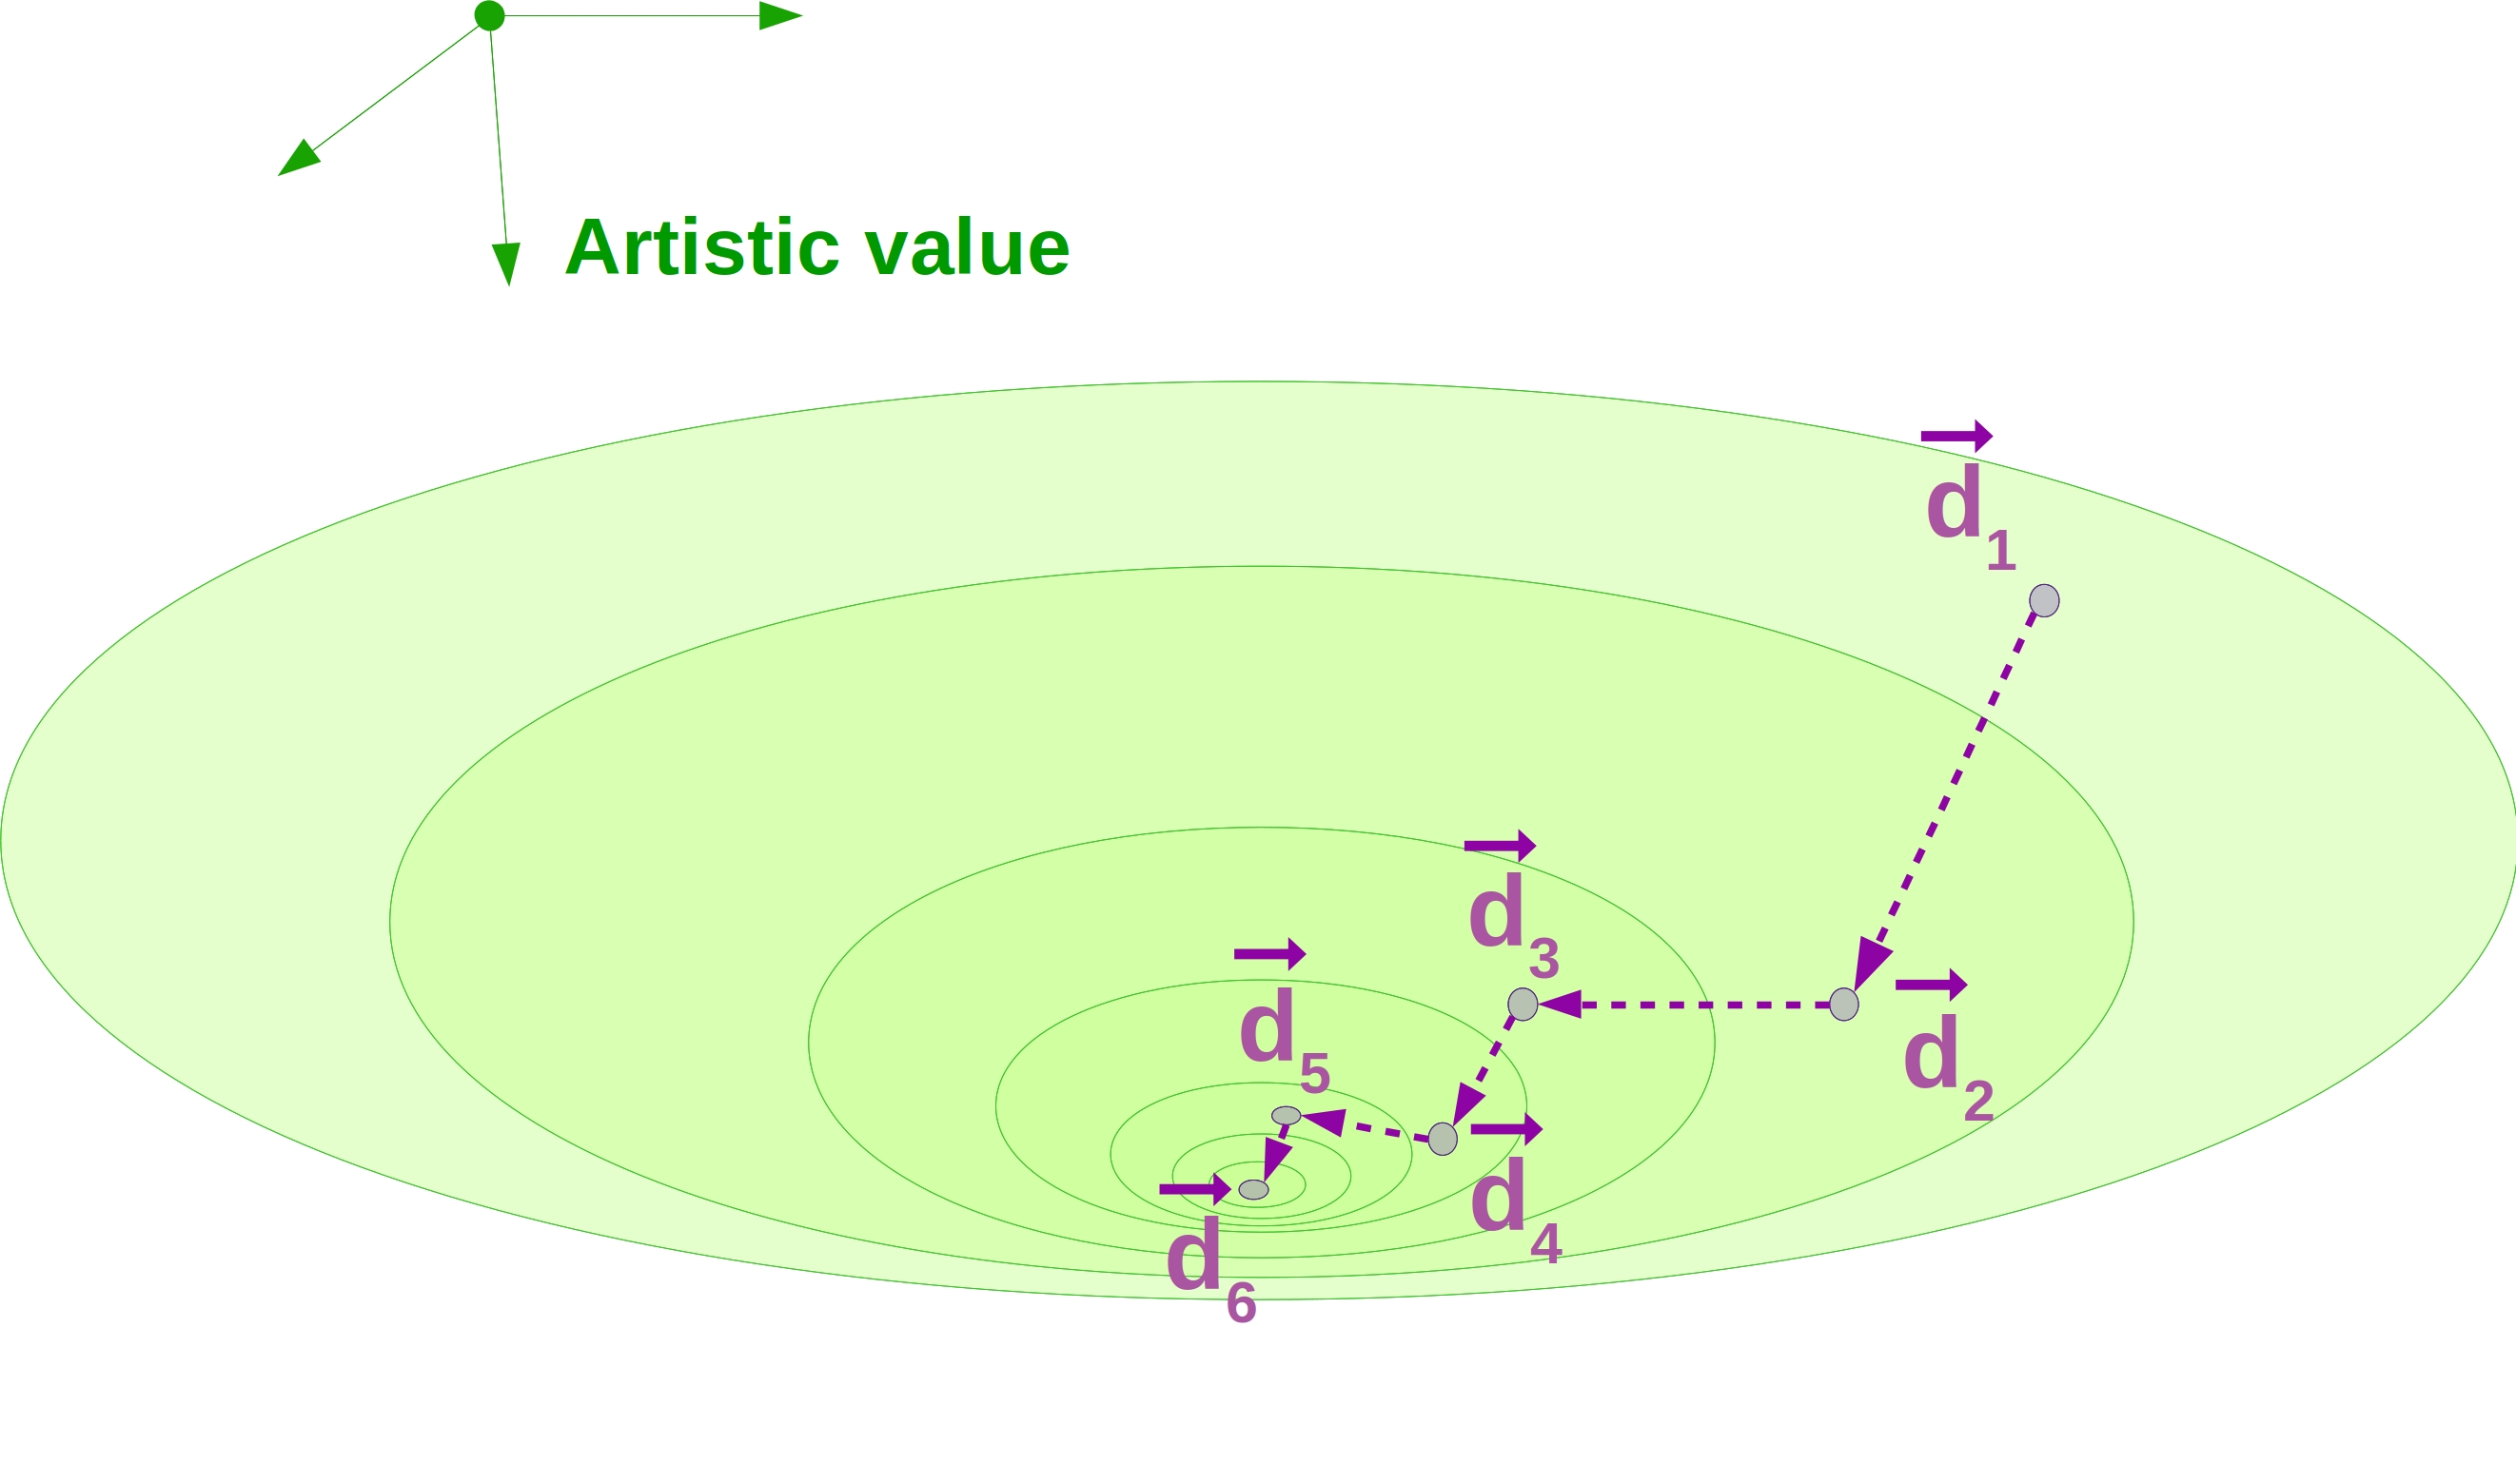
\includegraphics[width=0.6\textwidth]{/media/donkarlo/Elements/projs/research/assets/dependency-sequence-gradient-descent.jpg}
		\caption{dependencies from $d_1$ to $d_6$ where is the maximum artfulness} 
		\label{fig:dependency-gradient-descent}
	\end{figure}
	
	\section{Methodology} \label{sec:methodology}
		The methodology is composed of choosing a textual corpora from which a corpus of dependencies could be extracted and then introducing sequences with members of M such that they maximize the aesthetic  indexes introduced in Section \ref{sec:artfulness-indexes}.
		\subsection{Corpora building}
			\paragraph{Choosing textual Corpora} Since the objective of this proposal is prove that building literary text by complying with computationally defined aesthetic indexes is possible, the raw corpora should be chosen in such a way that it rarely conveys any aesthetic or literary senses. Otherwise the training sets turn to be biased and generating models can be alleged of solely reflecting the literary senses in the corpora. As such corpora such as Wikipedia may to turn to be applicable in such cases to wash such allegations.  
			\paragraph{Dependency parsing} To build a set such as M in Equation \ref{eq:space-of-possible-dependencies} dependency parsing techniques similar to \cite{de-marneffe-2014-universal-stanford-dependencies-a-cross-linguistic-typology} (or dependencies further than object-subject in \cite{nivre-2016-universal-dependencies-v1-a-multilingual-treebank-collection}) should be applied on the corpora. To some extent such approach is taking the Vladimir Propp's classical book on narratology \citep{propp-1968-morphology-of-the-folk-tale} which asserts characters and their permissible functions build stories. 
		
		\subsection{Semantic clustering} \label{sec:applications-of-semantic-classiication}
		 If a semantic vector space (such as \cite{mikolov-2013-distributed-representations-of-words-and-phrases-and-their-compositionality}) is generated in a  way that actions of a character(such as the protagonist) can shift the semantic class from one to the other, then  this could be used to mathematically define many aesthetic concepts. For example in Figure \ref{fig:semantical-class-shift} the effort of king's son to topple his father, shifts the semantic cloud from "Affection" to "Conspiracy". 
			
		
		\subsection{Artfulness indexes} \label{sec:artfulness-indexes}
		This document tries to introduce several aesthetic aspects of textual narratives and potential, computational methods of recognizing, generating or evaluating them. 
		
			\subsubsection{The Appeal of Ambiguity}
			Some studies have shown that ambiguity is an appealing constituent of an artifact \citep{muth-2015-the-appeal-of-challenge-in-the-perception-of-art-how-ambiguity-solvability-of-ambiguity-and-the-opportunity-for-insight-affect-appreciation}. For example, it is not determinable whether Mona Lisa is smiling and if she does, is it a bitter or a sweet smile? If the fate of a protagonist in a story ends close to two different (or even antonym) semantic classes, then such ambiguity provokes imagination (Figure \ref{fig:ambiguity}). 
			\citet{ono-2015-word-embedding-based-antonym-detection-using-thesauri-and-distributional-information} suggests a solution to detect antonyms using word-embedding. 
			\begin{figure}[h!]
				\centering
				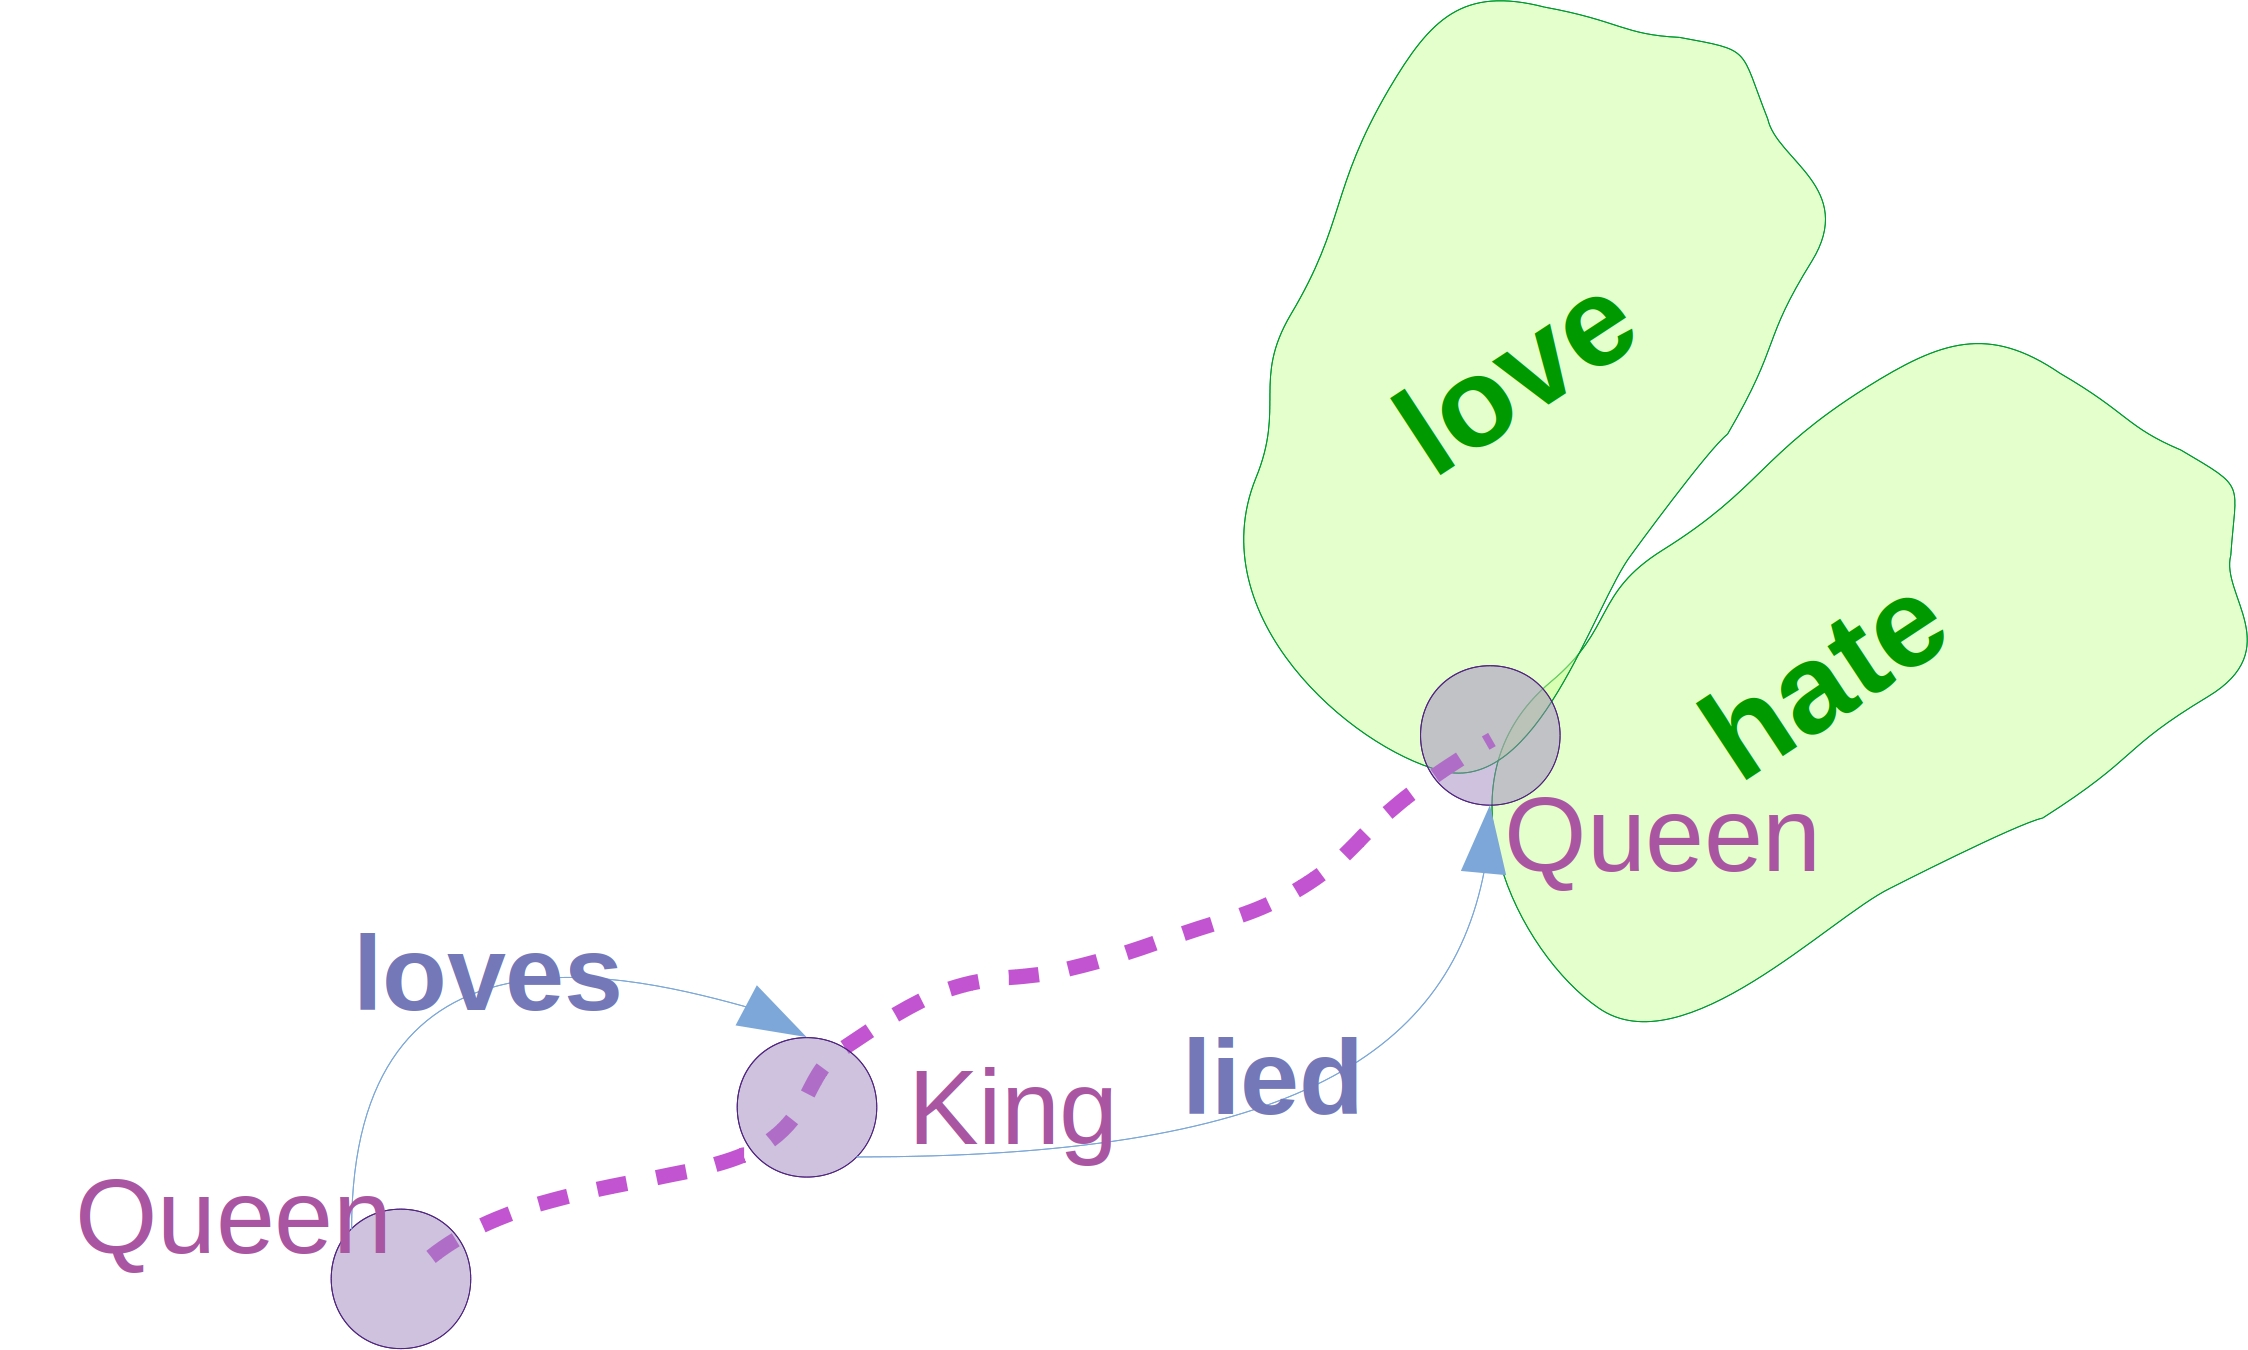
\includegraphics[width=0.6\textwidth]{../assets/ambiguity.jpg}
				\caption{A story which is ended in an ambiguity between "love" and "hate"} 
				\label{fig:ambiguity}
			\end{figure}
			\subsubsection{Valence, arousal and dominance of historical text}
			\citet{buechel-2016-feelings-from-the-past-adapting-affective-lexicons-for-historical-emotion-analysis}
			Whenever the course of the events takes the situation to a semantic class from which escaping is impossible then the audience mind deeply engages with imagining potential break outs. For example if the course of the events in the story, ends in a deep regret (\ref{fig:semantical-class-shift}), then however much a story character commits possible functions, s/he can not change the semantic class from regret to something different (such as happiness ....). Naturally, such endings engages the \textbf{imagination} of the audience(reader) to think of ways with which the character can release himself from such situations. 
			\begin{figure}[h!]
				\centering
				\includegraphics[width=1\textwidth]{../assets/reluctance-shift.jpg}
				\caption{Shifts to a space which is so huge that no other action can make any sentimental or semantical change in the narrative} 
				\label{fig:semantical-class-shift}
			\end{figure}
			With this regard, \citet{li-2017-inferring-affective-meanings-of-words-from-word-embedding} suggests an embedding particular to affective meaning which also includes the arousal and valence of the affection.
			
			\subsection{Transition between antonym semantic classes}
			Haiku is such a form that. it is usually formed of three verses which traverse from one meaning to its opposite and return back to the original one. 
			
			
			
			
			
			
			
			\subsubsection{Nostalgia} 
			In a semantic vector space, the rate of nostalgia introduced by a piece of text can be measured by the number of lexicons which are not explicitly mentioned in the text but are placed in a close neighborhood of the words which are already mentioned. This will implicitly remind the reader of unmentioned entities which provokes nostalgia. As such, semantic vector space tailor to previous knowledge of the reader must be formed. Such as forming it upon the literary texts he has already read. That is, if $n_p$ and $n_q$ are pieces of text of the same length, then the one which passes trough a denser space of words in a semantic vector space is more nostalgic and eventually a more artful text.  
			\begin{figure}[h!]
				\centering
				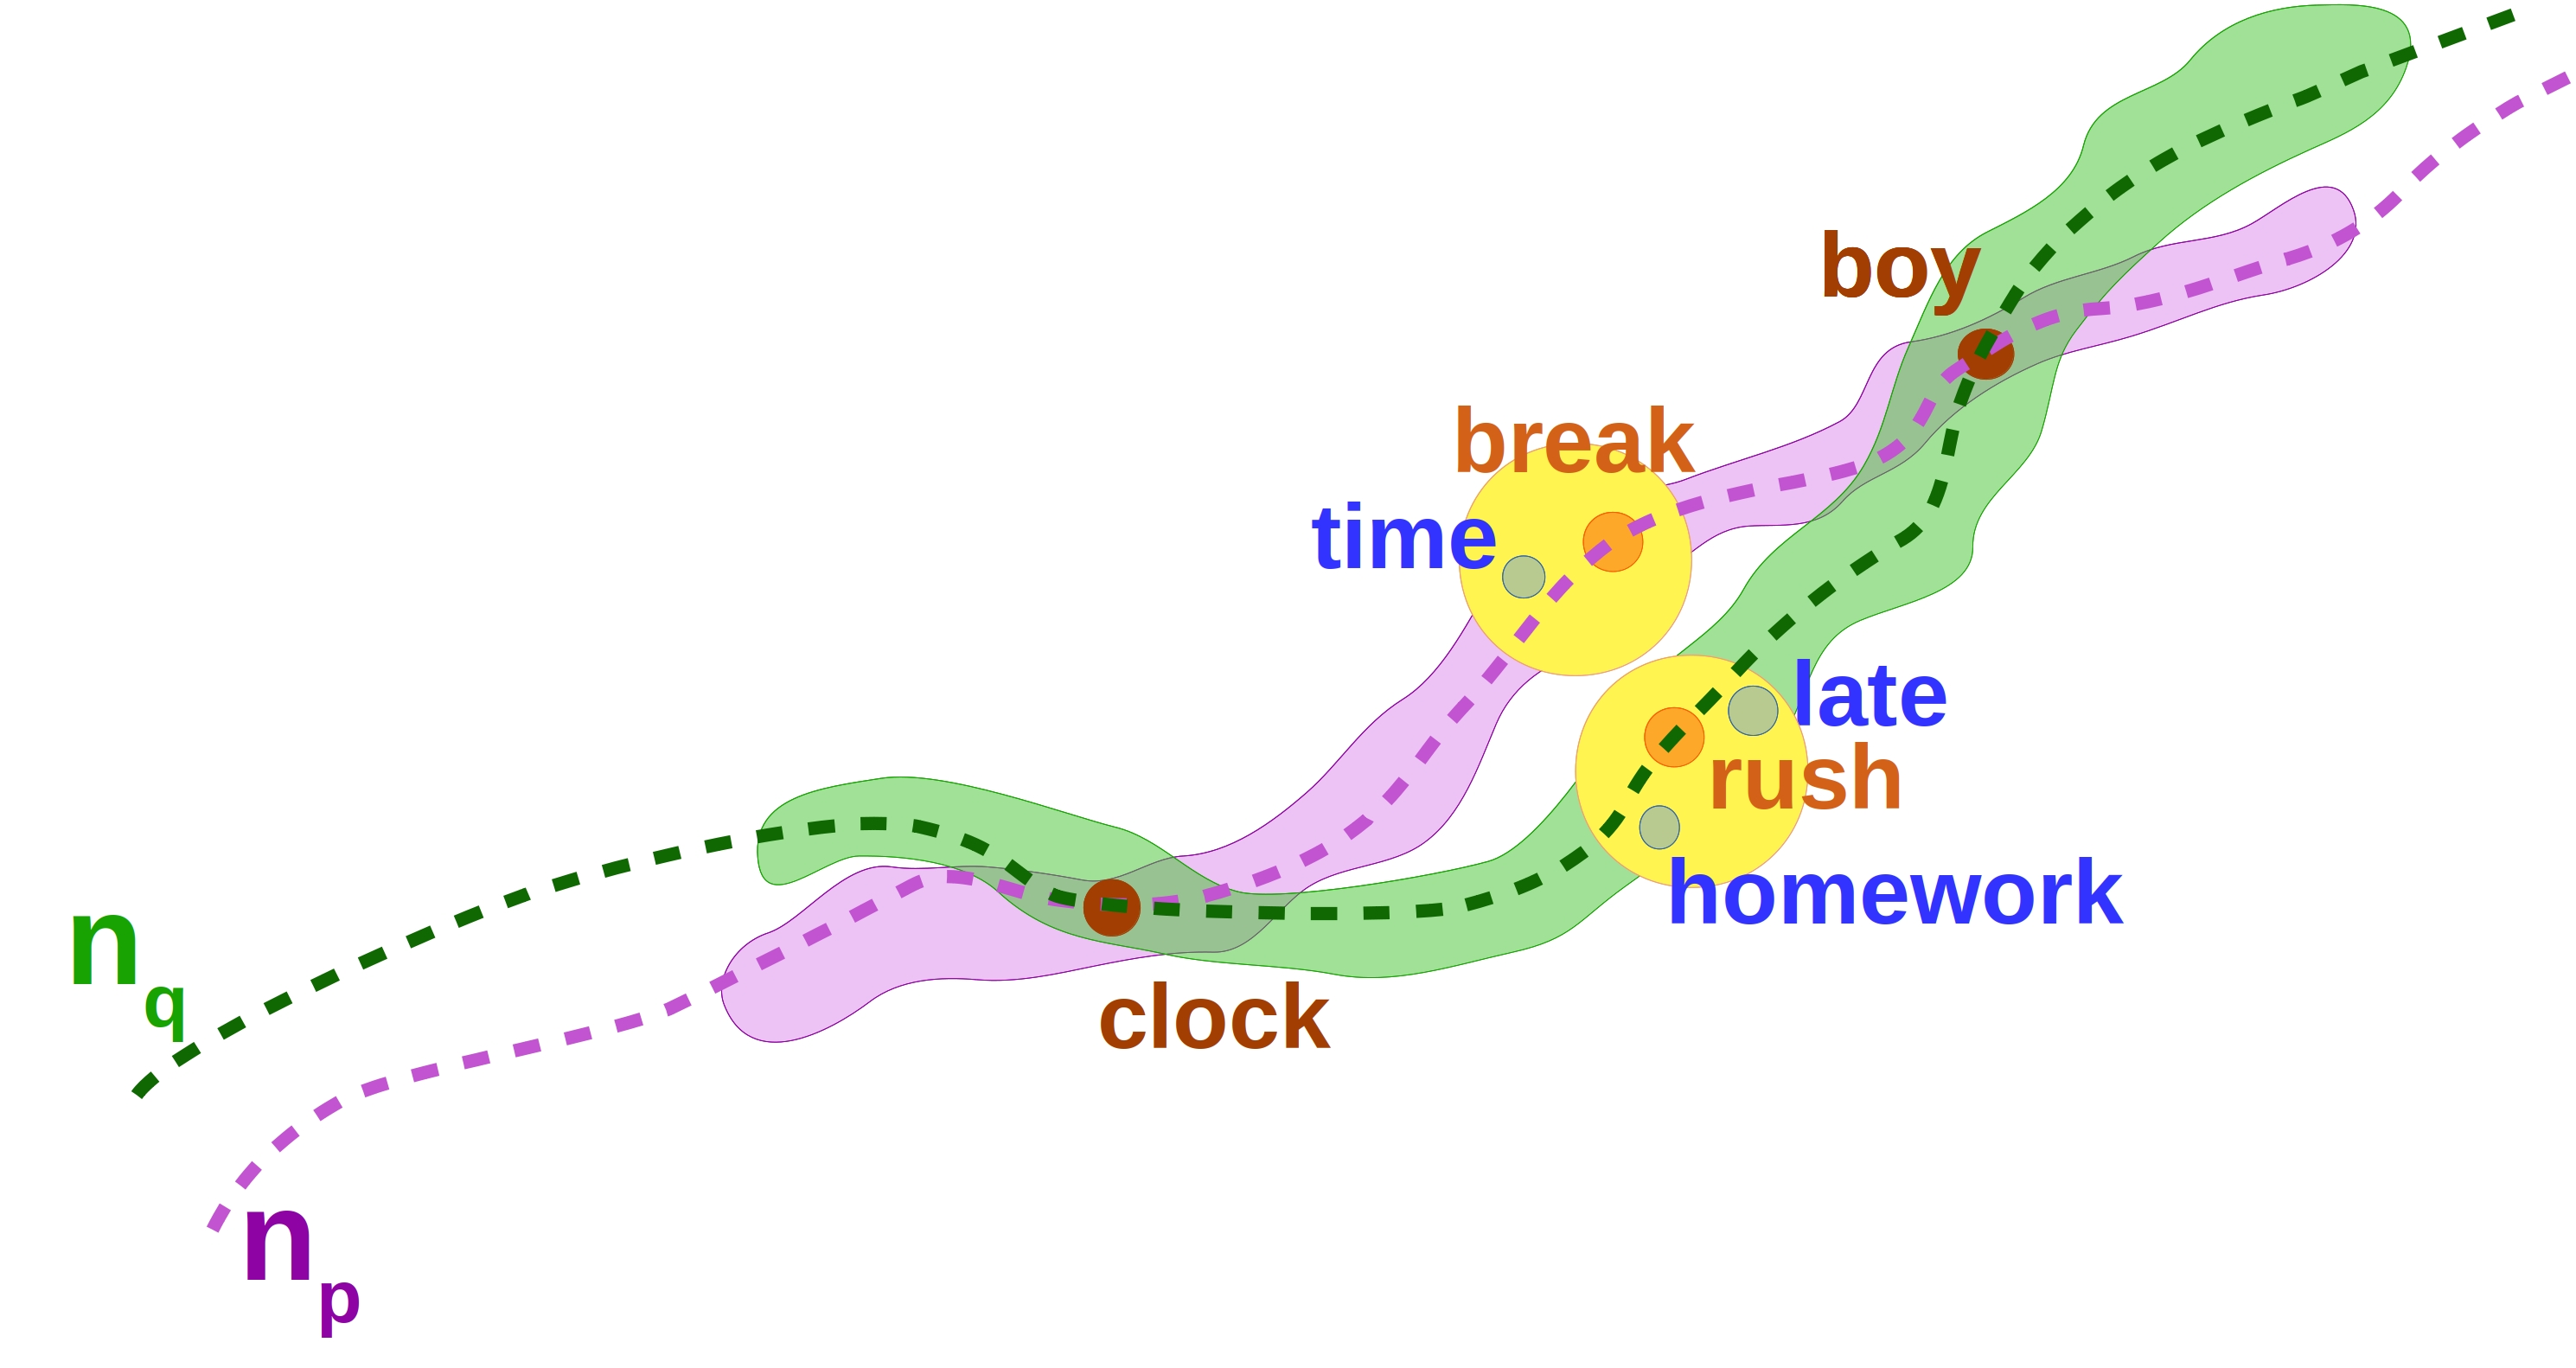
\includegraphics[width=1\textwidth]{../assets/cloud-evaluation.jpg}
				\caption{In this figure, $S=\{clock,boy\}$ is the set for which a text generator model should generate several candidate texts. Lets say the model has generated two candidate texts such as $N=\{n_q,n_p\}$ in which $n_q$="The \textbf{boy} looked at the \textbf{clock} and found that he has to \textbf{rush}" and $n_p$="The \textbf{clock} reminded the \textbf{boy} of a \textbf{break}". In other words $n_q=\{clock,rush,boy\}$ and $n_p=\{clock,break,boy\}$. The cloud around ${rush} \in n_q$ contains the semantic units $\{late,homework\}$ and the cloud around $"break" \in n_p$ contains $\{time\}$. Since $|n_q|=|n_s|=3$ then, $n_q$ is a better story(more nostalgic). Subjectively, it is more interesting because it may remind the reader a of rushing to do his/her homework when s/he was young for not being late!} 
				\label{fig:clouds-around-two-candidate-stories}
			\end{figure}
		
			\subsubsection{Adjectives and Adverbs}
			\citet{vecchi-2016-spicy-adjectives-and-nominal-donkeys-capturing-semantic-deviance-using-compositionality-in-distributional-spaces} focus on novel adjective in noun-phrases. They show that the extent to which an adjective alters the distributional representation of a noun it modifies is the most significant factor in determining the acceptability of the phrase.
			
			\subsubsection{Suspense}
			Suspense deals with keeping the audience(reader) worried about what is going to happen next. \citet{oneill-2011-toward-a-computational-framework-of-suspense-and-dramatic-arc} presents a suspense detection system based on the correlation between perceived likelihood of a protagonist’s failure and the amount of suspense reported by the audience.
			
			\subsubsection{Metaphors}\label{sec:metaphor}
			Metaphor bases one of the main columns of literature. As such, the more a piece of text contains metaphors, the more artful it appears.  \citet{mao-2018-word-embedding-and-wordnet-based-metaphor-identification-and-interpretation} suggests a method to identify metaphors applied in a text.    
			
			\subsubsection{Lexical choice} 
			Some lexical choices seem to be more aesthetic than others such as "vanish" versus "disappear" in a sentence such as "The baby vanishes into the cave" (This sentence is a causal output of the model suggested by \citet{mcintyre-2009-learning-to-tell-tales-a-data-driven-approach-to-story-generation}). It seems that the less frequent the synonym of a word is used, the more aesthetic it appears. 
			
			\subsubsection{Creativity}
			Creativity is the matter of being novel and unexpected. In recent years several methods have been developed to measure the amount of creativity introduced in a new product. For example, \citet{jordanous-2012-a-standardised-procedure-for-evaluating-creative-systems-computational-creativity-evaluation-based-on-what-it-is-to-be-creative} introduces 14 components of creativity. 
			Novelty can take many forms. One such form might appear in sentences such as "The baby vanishes into the cave". There is a perception that most of grammatically correct but semantically rare phrases can be considered artful. The reason might be the efforts the imagination has to make to establish natural relations between constituents of such bizarre phrases.
			
			
			
			
		
		\subsection{Generation and surface realization}
			\subsubsection{Generating the plan}\label{sec:plan-generation}
				Using the computational indexes introduced in Section \ref{sec:evaluation-indexes}, rank based or evolutionary methods will be used to select a subset of M in Equation \ref{eq:space-of-possible-relations} which maximizes the literary value of the text. It is worth mentioning that at generation phase no neural method is intended to be used since they all, more or less, imitate the compositions in the training data which contradict creativeness of an artifact even though in recent years application of Generative Adversarial Models are popular, yet this proposal looks for building all-novel literary text compositions. 
				\paragraph{Rank based}
					\citet{mcintyre-2009-learning-to-tell-tales-a-data-driven-approach-to-story-generation} uses a ranking method to rank different possible stories from a set such as M. 
				\paragraph{Evolutionary}
					\citet{mcintyre-2010-plot-induction-and-evolutionary-search-for-story-generation} uses an evolutionary method to to choose a subset from M as a sequence of a literary text. 
			\paragraph{Surface realization} There are many way for converting a plan to a text. Neural methods, particularly Long short-term memory networks \cite{hochreiter-1997-long-short-term-memory,sutskever-2014-sequence-to-sequence-learning-with-neural-networks} appear to be successful in converting the sequence of generated plan in Section \ref{sec:plan-generation} to a sequence of words. 
			
	\section{Evaluation and baselines}
		\subsection{Interestingness and story coherence}
		The baselines for interestingness and coherence are those presented in \citet{mcintyre-2009-learning-to-tell-tales-a-data-driven-approach-to-story-generation, mcintyre-2010-plot-induction-and-evolutionary-search-for-story-generation}.  
		\citet{xu-2018-a-skeleton-based-model-for-promoting-coherence-among-sentences-in-narrative-story-generation}
		\subsection{BLUE etc for surface generalization}
	
	\section{Time table}
		\begin{itemize}
			\item 6 months Choosing an unbiased corpora to develop semantic vector space methodology that can make an entity (an object or subject in Equation \ref{eq:space-of-possible-dependencies}) to new, relevant semantic classes upon committing actions.
			
			\item 9 Antonym leaps
			\item Appeal of ambiguity 
			\item Historical VAD for a class 
			\item Stochastic Gradient descent dependency sequence selection
			
		\end{itemize}
	
	
	\bibliography{/media/donkarlo/Elements/projs/research/refs}
\end{document}